% !TeX root = ../main.tex

\section{Degradación espacial de imágenes: PSF, emborronamiento y deconvolución}

Un telescopio real afecta a una imagen mediante una operación llamada convolución. En esta operación, la imagen que se obtiene es el resultado de la convolución de la imagen real con una función que se llama función de punto extendido, PSF (\textit{Point Spread Function}). La PSF describe cómo un punto de luz se extiende en la imagen debido a los efectos de desenfoque, aberraciones, difracción, etc. 

Matemáticamente se describe de esta manera:

\begin{equation}
    \label{eq:convolucion}
    d_{observado} = d_{real} * p
\end{equation}


En esta expresión, $d_{observado}$ es la imagen adquirida por el telescopio, $d_{real}$ es el objeto extenso original, y $p$ es la PSF del sistema óptico. A modo ilustrativo, se presenta la siguiente figura:


\begin{figure}[H]
    \centering
    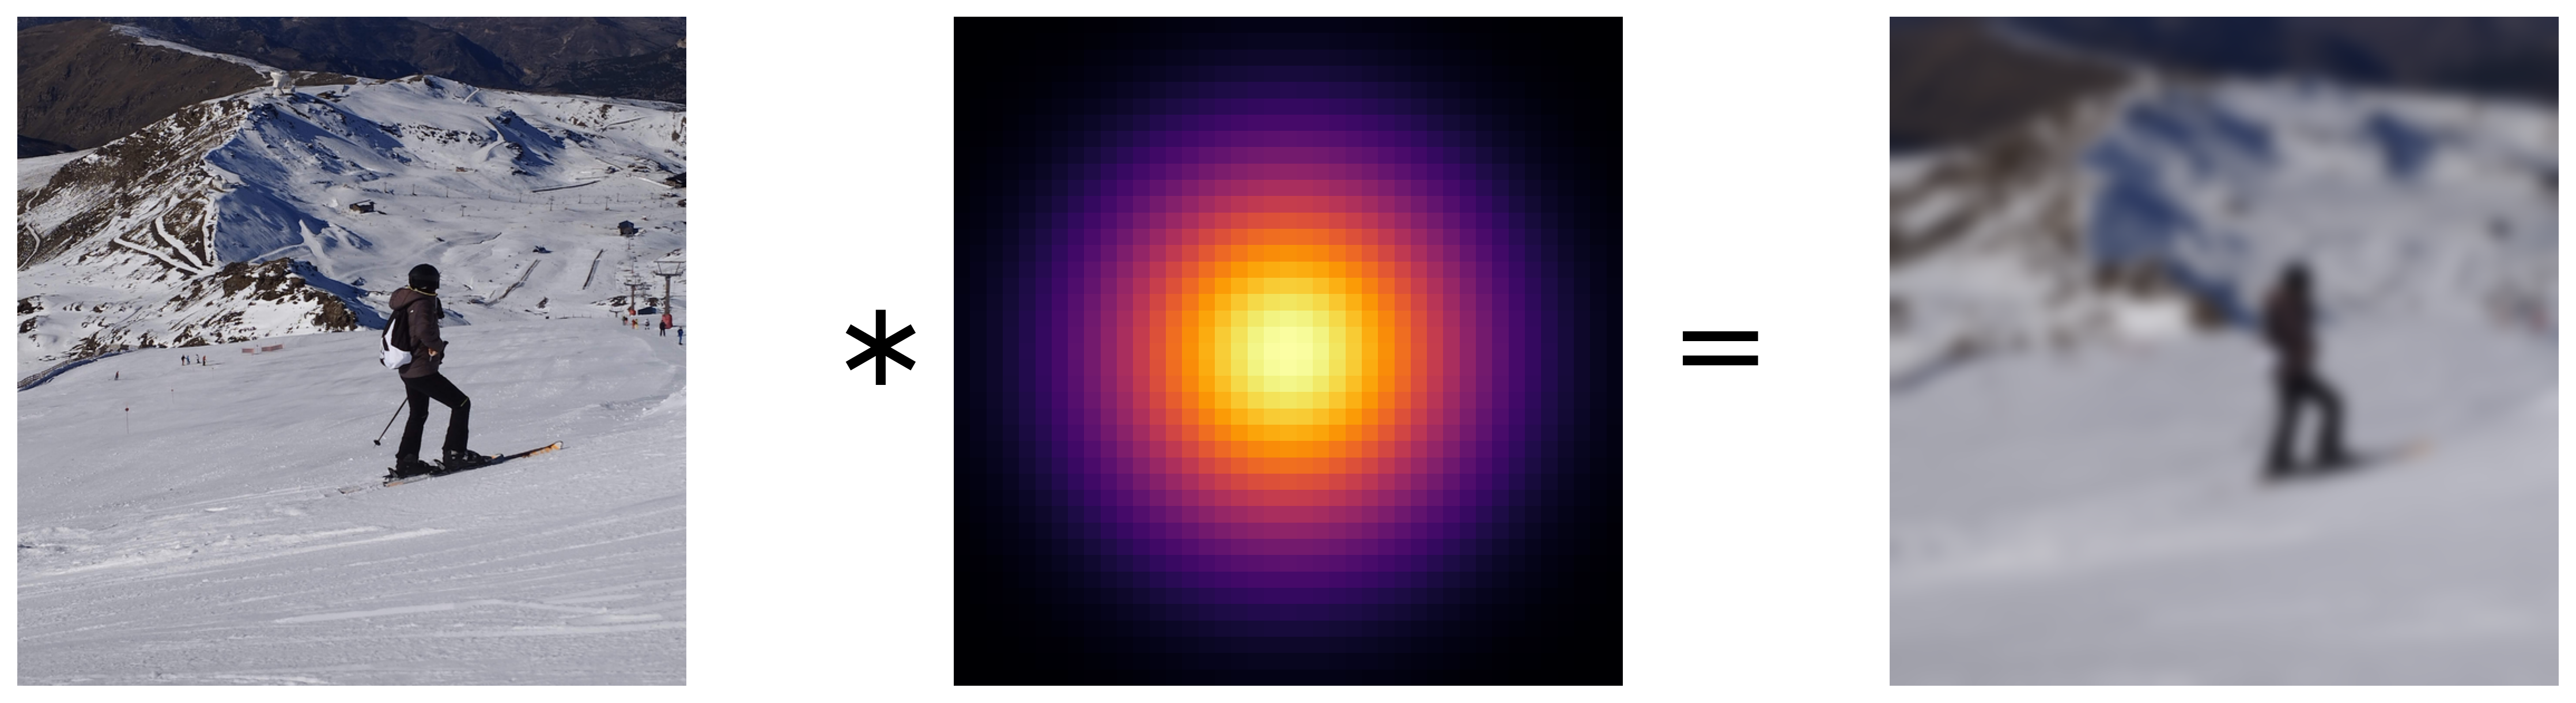
\includegraphics[width=0.8\textwidth]{img/ejemplo_degradacion.png}
    \caption{En esta imagen se muestra un ejemplo de cómo una imagen real se degrada al pasar por una lente. Se muestra de izquierda a derecha la imagen real ($d_{real}$), la PSF de la lente ($p$), y la imagen observada ($d_{observado}$).}
    \label{fig:ejemploConvolucion}
\end{figure}


Para hacer que este problema matemático sea más manejable, la técnica habitual es aplicar la Transformada de Fourier bidimensional. Esto nos permite pasar del dominio de la posición al dominio de las frecuencias espaciales. Si lo pensamos físicamente, estas frecuencias nos dicen cómo de rápido cambia la intensidad de la luz a lo largo de la imagen. Por ejemplo, las zonas donde la iluminación cambia poco a poco son las bajas frecuencias, mientras que los bordes marcados o los detalles más finos corresponden a las altas frecuencias. La gran ventaja matemática de saltar a este dominio es el Teorema de Convolución: gracias a él, una operación tan pesada como la convolución se convierte en una simple multiplicación, y viceversa.

\begin{equation}
    \label{eq:propFurier}
    \begin{split}
        \cdot &\Longrightarrow * \\
        * &\Longrightarrow \cdot
    \end{split}
\end{equation}

Sabiendo esto, si aplicamos la transformada a nuestra ecuación inicial (\ref{eq:convolucion}), el modelo en frecuencias queda mucho más limpio:

\begin{equation}
    \label{eq:convolucionFourier}
    D_{observado} = D_{real} \cdot P
\end{equation}

En este texto, la convención de notación emplea letras minúsculas para el dominio espacial y mayúsculas para el dominio de las frecuencias espaciales.

Si estuviéramos en un caso puramente ideal, bastaría con despejar directamente para encontrar $d_{real}$. Solo tendríamos que dividir la transformada de la imagen observada entre la de la PSF, llegando a la siguiente ecuación:

\begin{equation}
    \label{eq:deconvolucionIdeal}
    D_{real} = \frac{D_{observado}}{P}
\end{equation}

Finalmente, bastaría con deshacer la transformada (aplicar la inversa) para recuperar nuestra imagen $d_{real}$. Sin embargo, la realidad es bastante distinta, ya que las observaciones reales siempre arrastran ruido. Por ello, el modelo completo tiene que incluir este nuevo factor:

\begin{equation}
    \label{eq:convolucionRuido}
    d_{observado} = d_{real} * p + n
\end{equation}

donde $n$ representa el ruido añadido por el detector, la atmósfera u otras fuentes instrumentales. Al pasar al dominio de Fourier, la expresión queda:

\begin{equation}
    \label{eq:convolucionFourierRuido}
    D_{observado} = D_{real} \cdot P + N
\end{equation}

Con el ruido presente, la idea de despejar dividiendo directamente se vuelve inestable. El motivo es que al dividir entre $P$, también acabamos amplificando el ruido:

\begin{equation}
    \label{eq:deconvolucionRuido}
    D_{real} = \frac{D_{observado} - N}{P}
\end{equation}

Por tanto, la calidad de la deconvolución depende fuertemente de la relación señal-ruido.
